\documentclass[aspectratio=149]{beamer} %
\mode<presentation>
{
  \usetheme{CambridgeUS}       % or try default, Darmstadt, Warsaw, ...
  \usecolortheme{beaver} % or try albatross, beaver, crane, ...
  \usefonttheme{serif}     % or try default, structurebold, ...
  \setbeamertemplate{navigation symbols}{}
  \setbeamertemplate{caption}[numbered]
} 

\usepackage[italian]{babel}
\usepackage[utf8x]{inputenc}
\usefonttheme{structuresmallcapsserif}
\usepackage{palatino}
\usepackage{tikz}
\usepackage{amsmath}
\usepackage{verbatim}
\usepackage{booktabs}
\usepackage{graphicx}
\usepackage{subcaption}
\usepackage{lmodern}
\usepackage[scale=2]{ccicons}
\usepackage{xcolor}
\usepackage{multirow}
\usepackage{animate}
\usepackage{listings}
\usepackage{amsmath}
\usepackage{picture}
\usepackage[letterspace=150]{microtype}
\usepackage[absolute,overlay]{textpos}
\usepackage{tikzsymbols}
\usepackage{setspace}
\let\svthefootnote\thefootnote
\usepackage{animate}
\usepackage{xmpmulti}
\usepackage{tabularx}
\usepackage{array}
\setbeamersize{text margin left=5mm,text margin right=5mm}
\newcolumntype{P}[1]{>{\centering\arraybackslash}p{#1}}
\textheight 1in
\newcommand\Factor{1.2}
\newenvironment{slide}{\begin{frame}[fragile,environment=slide]}{\end{frame}}
\AtBeginSection[]{
	\begin{frame}
		\setbeamercolor{coloredboxstuff}{}
		\vfill
		\centering
		\begin{beamercolorbox}[sep=8pt,center,shadow=true,rounded=true]{coloredboxstuff}
			\large\textsc\insertsectionhead\par%
		\end{beamercolorbox}
		\vfill
	\end{frame}
}


\AtBeginSubsection[] % Do nothing for \subsection*
{
	\begin{frame}
		\vfill
		\centering
		\begin{beamercolorbox}[sep=8pt,center,shadow=true,rounded=true]{title}
			\bfseries\insertsubsectionhead\par%
		\end{beamercolorbox}
		\vfill
	\end{frame}
}

%\renewcommand\baselinestretch{1.5}

\usepackage{Sweave}
\begin{document}
\Sconcordance{concordance:03-LaTeX.tex:03-LaTeX.Rnw:%
1 69 1 1 0 1 60 1 28 1 -87 299 1 1 4 1 2 72 1 1 3 16 0 1 2 13 1 1 2 6 1 %
1 4 25 0 1 2 27 1 1 2 4 0 1 2 72 1}


\title{03-\LaTeX}
\author{Ottavia M. Epifania}
\date{Università di Padova}
\titlegraphic{
    
\includegraphics[width=2cm]{C:/Users/huawei/OneDrive/Documenti/GitHub/CorsoRmarkdown/man/arca_logo.png}
}

\begin{frame}
\maketitle
\end{frame}

\section{\LaTeX, \texttt{Sweave}, \texttt{knitr}}

\begin{frame}

\begin{itemize}
\item Per scrivere documenti importanti che rimangano bene sempre e comunque è il software migliore

\item Per produrre file LaTeX, si utilizza \texttt{Sweave} $\rightarrow$ estensione \texttt{.Rnw}

\item Per aprire un file  \texttt{.Rnw}: File $\rightarrow$ New File $\rightarrow$ R Sweave 

\item Se volete usare un file \LaTeX indipendente da \texttt{R}, provate a usare TeXStudio (\url{https://www.texstudio.org/})
\end{itemize}


\end{frame}


\begin{frame}{Attenzione!}
 
 Se si utilizza \texttt{Sweave} l'integrazione con i chunk di codice è un po' difficoltosa.

Per  poter integrare \LaTeX e R, andate su Tools $\rightarrow$ Global options: 

\centering
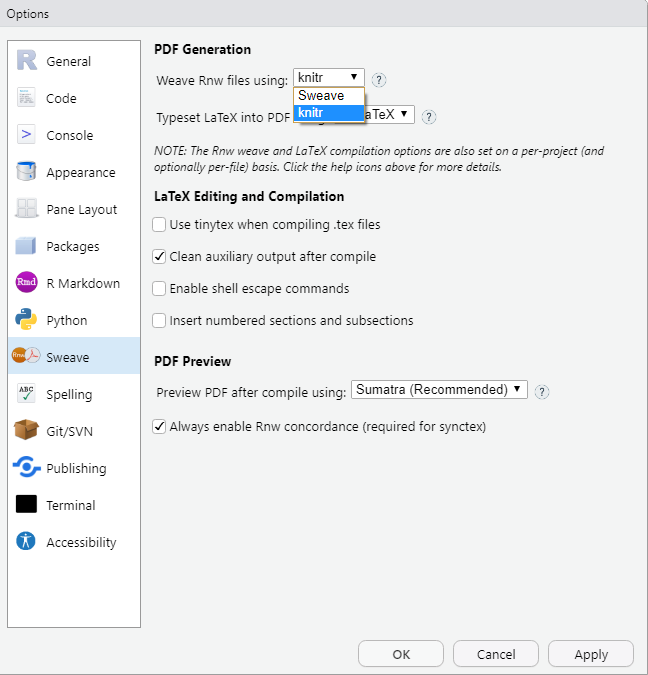
\includegraphics[width=.60\linewidth]{img/knitr.png}

\end{frame}

\section{Impostare un documento \LaTeX}
\subsection*{Articolo o report}

	\begin{slide}
		\begin{scriptsize}
			\begin{verbatim}
			\documentclass[12pt, a4paper, titlepage]{article}
			\usepackage{amsmath} %equazioni e simboli matematici
			\usepackage{xcolor} %colori
			\usepackage{graphicx} %immagini
			\usepackage{subcaption} %etichette delle immagini
			\usepackage{multicol} %gestione delle colonne
			\usepackage{tabularx} %larghezza delle colonne
			\usepackage{apacite} %gestisce le citazioni
			\bibliographystyle{apacite} % formattazione delle citazioni
			
			\title{Titolo di esempio}
			\author{Jane Doe}
\usepackage{Sweave}
\begin{document}
				\maketitle %crea pagina del titolo
				\begin{abstract} %pagina dell'abstract
				\end{abstract}
				\section{Titolo della sezione}
				\subsection{Titolo della sottosezione}
				\subsubsection{Titolo della sotto-sottosezione}
				\paragraph{Titolo del paragrafo}
				\bibliography{bibFile.bib} %bibliografia
			\end{document}
			\end{verbatim}
		\end{scriptsize}
	\end{slide}

\subsection*{Presentazione}
\begin{slide}
	
	\begin{scriptsize}
			\begin{verbatim}
			\documentclass{beamer} %classe del documento
			\usetheme{default} % template del documento
			\usepackage{multirow} %per le tabelle
			\usepackage{verbatim} %per scrivere il codice ``raw''
			\usepackage{xcolor} %per i colori
			\usepackage{listings} %per plottare i grafici R
			
			\title{Beamer Template} %Titolo
			\author{TeXstudio Team} %autori della presentazione
\usepackage{Sweave}
\begin{document}
				\begin{frame}[plain] 
					\maketitle
				\end{frame}
				
				\begin{frame}{Titolo della diapositiva}
					
				\end{frame}
			\end{document}
		\end{verbatim}
	\end{scriptsize}

\begin{small}
A questa pagina \url{https://deic.uab.cat/~iblanes/beamer_gallery/} si trovano tutte le posibili combinazioni di stili per le slides. Enjoy
\end{small}

\end{slide}

\section{Formattazione}

\begin{frame}[fragile]
	
	\begin{columns}[T]
		\column[T]{.50\linewidth}
		
		\begin{verbatim}
			
			\emph{Corsivo}
			
			\textbf{Grassetto}
			
			\underline{Sottolineato}
			
			\textcolor{red}{Parola colorata}
			
			\textbf{\textcolor{red}{Parola}}
			
		\end{verbatim}
	
	\column[T]{.50\linewidth}
	\centering
	
	\vspace{5mm}
		\emph{Corsivo}
	\vspace{5mm}
	
	\textbf{Grassetto}
	\vspace{5mm}
	
	\underline{Sottolineato}
	\vspace{5mm}
	
	\textcolor{red}{Parola colorata}
	\vspace{5mm}
	
	\textbf{\textcolor{red}{Parola}}
	\end{columns}
	
\end{frame}

\begin{frame}[fragile]

\begin{columns}[T]
\column{.50\linewidth}
\begin{small}
\begin{verbatim}
\Huge{Huge}

\huge{huge}

\LARGE{LARGE}

\Large{Large}

\large{large}

\normalsize{normalsize}

\footnotesize{footnotesize}

\scriptsize{scriptsize}

\tiny{tiny}
\end{verbatim}
\end{small}


\column{.50\linewidth}

\Huge{Huge}
\vspace{3mm}

\huge{huge}
\vspace{3mm}

\LARGE{LARGE}
\vspace{3mm}

\Large{Large}
\vspace{3mm}

\large{large}
\vspace{3mm}

\normalsize{normalsize}
\vspace{3mm}

\footnotesize{footnotesize}
\vspace{3mm}

\scriptsize{scriptsize}
\vspace{3mm}

\tiny{tiny}

\end{columns}

\end{frame}

\begin{frame}[fragile]{Elenchi}
	
	\begin{columns}[T]
		\column[T]{.50\linewidth}
			Puntati: 
		
		\begin{verbatim}
			\begin{itemize}
				\item Guanciale
				\item Pecorino
				\item Uovo
			\end{itemize}
		\end{verbatim}
		
		Numerati: 
		
		\begin{verbatim}
			\begin{enumerate}
				\item Carbonara
				\item Gricia
				\item Amatriciana
			\end{enumerate}
		\end{verbatim}
	
		\column[T]{.50\linewidth}
		
			Puntati: 
		
		\vspace{5mm}
	%	\begin{verbatim}
			\begin{itemize}
				\item Guanciale
				\item Pecorino
				\item Uovo
			\end{itemize}
	%	\end{verbatim}
		
			\vspace{5mm}
		Numerati: 
		\vspace{5mm}
		
	%	\begin{verbatim}
			\begin{enumerate}
				\item Carbonara
				\item Gricia
				\item Amatriciana
			\end{enumerate}
	%	\end{verbatim}
	\end{columns}
	
\end{frame}

\begin{frame}[fragile]
Le colonne nelle presentazioni (2 colonne): 

\begin{verbatim}
\begin{columns} %l'ambiente per le colonne
\column{.50\linewidth} %prima colonna larga la metà della slide
Testo nella prima colonna
\column{.50\linewidth} %seconda colonna larga la metà della slide
Testo nella seconda colonna
\end{columns}
\end{verbatim}

\pause

\begin{columns} %l'ambiente per le colonne
\column{.50\linewidth} %prima colonna larga la metà della slide
Testo nella prima colonna
\column{.50\linewidth} %seconda colonna larga la metà della slide
Testo nella seconda colonna
\end{columns}
\end{frame}

\section{Bibliografia e citazioni}

\begin{frame}[fragile]
\begin{figure}
		
		\centering
		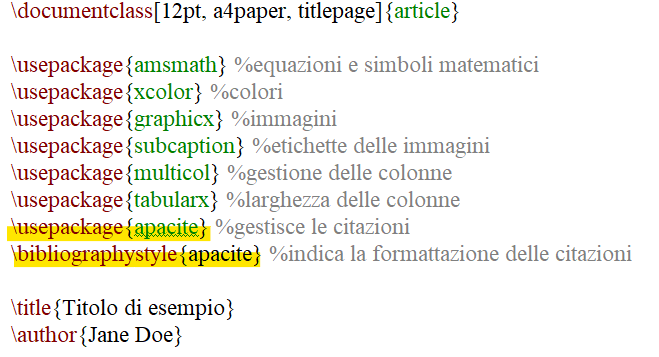
\includegraphics[width=.7\linewidth]{img/bib1.png}
	
\end{figure}

Per poterla usare: 

\begin{verbatim}
	\bibliography{file.bib}
\end{verbatim}

\end{frame}

\begin{frame}{Come si cita}
		\begin{figure}
			
			\centering
			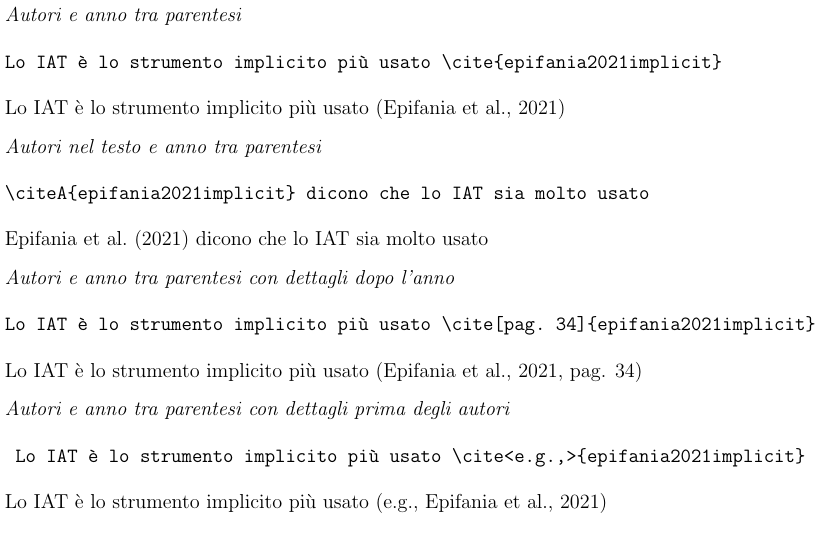
\includegraphics[width=.9\linewidth]{img/bibExample.png}
			
		\end{figure}
		
\end{frame}

\section{Figure e plot}

\begin{frame}[fragile]
	
		\begin{small}
			\begin{verbatim}
			\begin{figure}
				\caption{Me, right now.}
				\label{fig:happyCat}
				\centering
				
\includegraphics[width=.50\linewidth]{img/cat.jpg}
			\end{figure}
		\end{verbatim}
		\end{small}
		

\begin{footnotesize}
	\begin{verbatim}
		In figura \ref{fig:happyCat} si può vedere l'entusiasmo per [...]
	\end{verbatim}
\end{footnotesize}

\pause
In figura \ref{fig:happyCat} si può vedere l'entusiasmo per il corso di RMarkdown.
	\begin{figure}
	\caption{Me, right now.}
	\label{fig:happyCat}
	\centering
	
\includegraphics[width=.30\linewidth]{C:/Users/huawei/OneDrive/Documenti/GitHub/CorsoRmarkdown/slides/03 - LaTeX/img/cat.jpg}
\end{figure}
\end{frame}

\subsection*{Plot}

\begin{frame}[fragile]


Nell'header del documento bisogna aggiungere un pacchetto: 

	\begin{small}
		\begin{verbatim}
			\usepackage{listings}
		\end{verbatim}
	\end{small}

Per fare il grafico:

	\begin{small}
		\begin{verbatim}
		\begin{figure}
		\caption{Un plot}
		\label{fig:plot}
       <<echo=FALSE, fig=TRUE, width=3, height=2>>=
       library(ggplot2)
       ggplot(cars, aes(x=speed, y=dist, size =dist, color =speed)) + geom_point() +
       theme_bw() + theme(legend.position = "none")
      @
		 \end{figure}
		\end{verbatim}
	\end{small}

\end{frame}

\begin{frame}[fragile]

\begin{verbatim}
 In figura \ref{fig:plot} c'è un plot.
\end{verbatim}

In figura \ref{fig:plot} c'è un plot.

\begin{figure}
\caption{Un grafico}
\label{fig:plot}
\centering
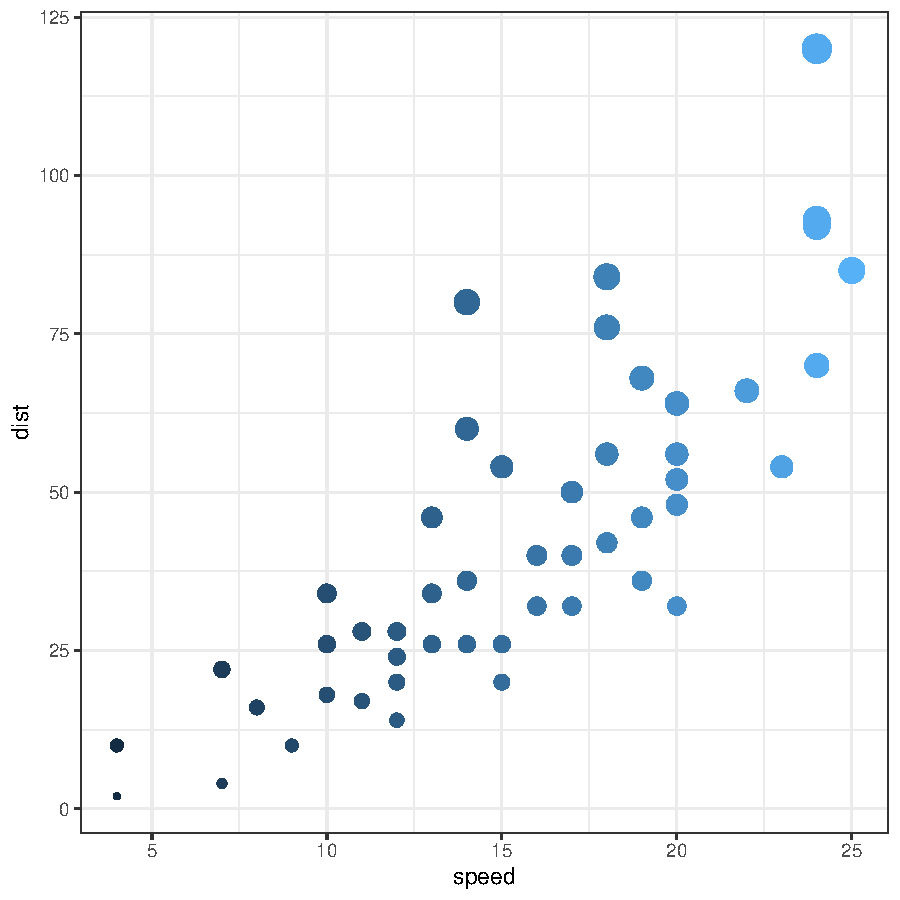
\includegraphics{03-LaTeX-001}

\end{figure}
\end{frame}


\section{Tabelle}

\begin{frame}[fragile]
	
	La sintassi (molto comoda) per generare le tabelle: 
	
	\begin{columns}
		\column[T]{.50\linewidth}
		
		\begin{footnotesize}
			\begin{verbatim}
			\begin{table}[]
				\caption{Una tabella}
				\label{tab:tabella}
			\begin{tabular}{|l|l|}
				\hline
				Colonna 1 & Colonna 2  \\ \hline
				1         & 2       \\   \hline
				4         & 5         \\  \hline
			\end{tabular}
		\end{table}
		\end{verbatim}
		\end{footnotesize}
		
		\column[T]{.50\linewidth}
		
			\begin{table}[]
				\caption{Una tabella}
				\label{tab:tabella}
			\begin{tabular}{|l|l|}
				\hline
				Colonna 1 & Colonna 2  \\ \hline
				1         & 2       \\   \hline
				4         & 5         \\  \hline
			\end{tabular}
		\end{table}
		
	\end{columns}
	
	\vspace{3mm}
	
	\begin{small}
			\begin{verbatim}
			Vediamo quanto sia comodo generare Tabella \ref{tab:tabella}.
		\end{verbatim}
	\end{small}


Vediamo quanto sia comodo generare Tabella \ref{tab:tabella}. \url{https://www.tablesgenerator.com/} aiuta a generare tabelle senza impazzire... 

\centering

MA 
	
\end{frame}

\begin{frame}[fragile]
	Ma siccome siamo su \texttt{R}, usiamolo: 
	
	\texttt{xtable}
	
	\begin{verbatim}
		<<chunk, echo=FALSE, results=tex, message=FALSE>>=
		library(xtable)
xtable(head(cars), caption = "Tabella")
		@
	\end{verbatim}
	
% latex table generated in R 4.2.0 by xtable 1.8-4 package
<<<<<<< HEAD
% Thu May 19 13:41:35 2022
=======
% Fri May 20 11:25:03 2022
>>>>>>> a6f15b3880c29f61c584cdd958fa7db2db12ae72
\begin{table}[ht]
\centering
\begin{tabular}{rrr}
  \hline
 & speed & dist \\ 
  \hline
1 & 4.00 & 2.00 \\ 
  2 & 4.00 & 10.00 \\ 
  3 & 7.00 & 4.00 \\ 
  4 & 7.00 & 22.00 \\ 
  5 & 8.00 & 16.00 \\ 
  6 & 9.00 & 10.00 \\ 
   \hline
\end{tabular}
\caption{Tabella} 
\end{table}
\end{frame}


\begin{frame}[fragile]

\texttt{stargazer}:

\begin{footnotesize}
	\begin{verbatim}
		<<model, echo=FALSE, results=tex>>=
    library(stargazer)
    model = lm(dist ~ speed, data = cars)
    stargazer(model, type="latex", header=FALSE, title="Modello", 
              label = "tab:modello")
	\end{verbatim}

\end{footnotesize}

\tiny

\begin{table}[!htbp] \centering 
  \caption{Modello} 
  \label{tab:modello} 
\begin{tabular}{@{\extracolsep{5pt}}lc} 
\\[-1.8ex]\hline 
\hline \\[-1.8ex] 
 & \multicolumn{1}{c}{\textit{Dependent variable:}} \\ 
\cline{2-2} 
\\[-1.8ex] & dist \\ 
\hline \\[-1.8ex] 
 speed & 3.932$^{***}$ \\ 
  & (0.416) \\ 
  & \\ 
 Constant & $-$17.579$^{**}$ \\ 
  & (6.758) \\ 
  & \\ 
\hline \\[-1.8ex] 
Observations & 50 \\ 
R$^{2}$ & 0.651 \\ 
Adjusted R$^{2}$ & 0.644 \\ 
Residual Std. Error & 15.380 (df = 48) \\ 
F Statistic & 89.567$^{***}$ (df = 1; 48) \\ 
\hline 
\hline \\[-1.8ex] 
\textit{Note:}  & \multicolumn{1}{r}{$^{*}$p$<$0.1; $^{**}$p$<$0.05; $^{***}$p$<$0.01} \\ 
\end{tabular} 
\end{table} 
\end{frame}


\subsection*{Cross-reference delle tabelle}


\begin{frame}[fragile]

\texttt{xtable}:

\begin{footnotesize}
\begin{verbatim}
  <<tabella, echo=FALSE, results=tex, message=FALSE>>=
	library(xtable)
  print(xtable(head(cars), caption = "Tabella delle macchine",
             label = "tab:macchine"))
  @
\end{verbatim}


% latex table generated in R 4.2.0 by xtable 1.8-4 package
<<<<<<< HEAD
% Thu May 19 13:41:35 2022
=======
% Fri May 20 11:25:03 2022
>>>>>>> a6f15b3880c29f61c584cdd958fa7db2db12ae72
\begin{table}[ht]
\centering
\begin{tabular}{rrr}
  \hline
 & speed & dist \\ 
  \hline
1 & 4.00 & 2.00 \\ 
  2 & 4.00 & 10.00 \\ 
  3 & 7.00 & 4.00 \\ 
  4 & 7.00 & 22.00 \\ 
  5 & 8.00 & 16.00 \\ 
  6 & 9.00 & 10.00 \\ 
   \hline
\end{tabular}
\caption{Tabella delle macchine} 
\label{tab:macchine}
\end{table}

\begin{verbatim}
In Tabella \ref{tab:macchine} c'è il dataset \texttt{cars}
\end{verbatim}

In Tabella \ref{tab:macchine} c'è il dataset \texttt{cars}

\end{footnotesize}



\end{frame}


\begin{frame}[fragile]
\texttt{stargazer}:

\begin{verbatim}
In Tabella \ref{tab:modello} ci sono i risultati di un modello di [..]
\end{verbatim}

In Tabella \ref{tab:modello} ci sono i risultati di un modello di regressione

\end{frame}



\section{Chunk di codice}

\begin{frame}[fragile]

I chunk di codice si ottengono con la classica combo \texttt{ctrl + alt + i}

\begin{verbatim}
 <<nome, echo= TRUE, eval = TRUE, fig = TRUE>>=

 @
\end{verbatim}

Funzionano esattamente come i chunk in \texttt{RMarkdown} con qualche piccola accortezza (tipo per mettere le immagini e regolarne la grandezza)

\begin{verbatim}

\end{verbatim}

Permette di richiamare i risultati del codice nel testo
\end{frame}

\begin{frame}[fragile]

Calcoliamo la media della velocità e la assegnamo all'oggetto \texttt{x}:

\begin{Schunk}
\begin{Sinput}
> x = mean(cars$speed)
\end{Sinput}
\end{Schunk}

Per riportare la velocità media nel testo: 

\begin{verbatim}
La velocità media è di \ Sexpr{x}
\end{verbatim}

La velocità media è di 15.4

\end{frame}

\section{Equazioni e simboli matematici}

\begin{frame}[fragile]
	Funziona quasi esattamente come \texttt{RMarkdown}. 
	
	\$2 + 3\$ è la sintassi per scrivere equazioni in linea: $2+3$
	
	\$\$2+3\$\$ è la sintassi per scrivere equazioni isolate: $$2+3$$

Si può usare anche l'ambiente \texttt{equation} per le equazioni isolate e volendo numerate


\begin{columns}
\column[T]{.50\linewidth}

\centering
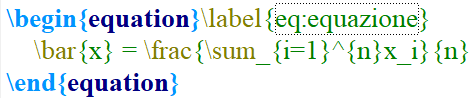
\includegraphics[width=\linewidth]{img/eq.png}

\begin{verbatim}
In Equazione \ref{eq:equazione} si calcola la media
\end{verbatim}

\column[T]{.50\linewidth}
\begin{equation}\label{eq:equazione}
	\bar{x} = \frac{\sum_{i=1}^{n}x_i}{n}
\end{equation}


In Equazione \ref{eq:equazione} si calcola la media

\end{columns}
	
\end{frame}


\begin{frame}[fragile]

Se si vuole integrare un'equazione con i risultati di un chunk, è molto semplice: 

\begin{small}
\begin{verbatim}
La velocità media è: $\bar{x} = \frac{\sum_{i=1}^{n} x_i}{n} = \ Sexpr{x}$
\end{verbatim}
\end{small}


La velocità media è: $\bar{x} = \frac{\sum_{i=1}^{n} x_i}{n} = 15.4$

\end{frame}

\section{Last but not least}

\begin{slide}

In un certo senso, \texttt{Sweave} è più sensibile da usare e bisogna avere delle accortezze in più: 

Se si sta facendo una presentazione (quindi si usa la classe \texttt{beamer}): 

\begin{verbatim}
    \begin{frame}[fragile]
    <<echo=TRUE, eval=TRUE>>=
    summary(cars)
    @
    \end{frame}
\end{verbatim}

Senza quel \texttt{[fragile]} non solo non si vede l'output di \texttt{R} ma proprio non si riesce a compilare il file perché risulta un errore

\end{slide}

\end{document}
